% !TeX root = ../main.tex
\section{Cohomology} % (fold)
\label{sec:cohomology}

A \textbf{cochain complex} is a sequence $\C = (C^*, \delta_*)$ of $\R$-modules $C^k$ consisting of \textbf{cochains} and module homomorphisms known as \textbf{coboundary maps} $\delta_k:C^k\to C^{k+1}$.
As in homology we have the property that $\delta_{k+1}\circ\delta_k = 0$ for all $k$, leading to a familiar definition of the \textbf{cohomology} of $\C$
\[ H^k(\C) = \ker\delta_k/\im\delta_{k-1}.\]
The equivalence classes of $H^k(\C)$ consist of \textbf{$k$-cocycles}: elements of $\ker\delta_k$ that differ by a \textbf{$k$-coboundary} in $\im\partial_{k-1}$.
Such cocycles are said to be \textbf{cohomologous} if they belong to the same equivalence class in $H^k(\C)$.

The simplest construction of a cochain complex is to dualize a chain complex.
For a simplicial complex $K$ with chain complex $(C_*,\partial_*)$ define $C^k(K)$ to be the module of homomorphisms $\psi:C_k\to\R$.
The coboundary maps $\delta_k$ are defined for cochains $\psi:C_k\to\R$ and $k$-simplices $\sigma\in K$ as
\[\delta_k\psi(\sigma) = \psi(\partial_k\sigma).\]

\subsection{Representative Cycles and Cocycles}

We can find a basis for each homology group $H_p(K)$ and cohomology group $H^p(K)$ consisting of $p$-cycles and $p$-cocycles, respectively.
In general, $p$-cycles represent $p$-dimensional holes in the simplicial complex $K$, where $p$-cocycles can be understood as ``blocking chains.''

\begin{figure}[htbp]
\centering
    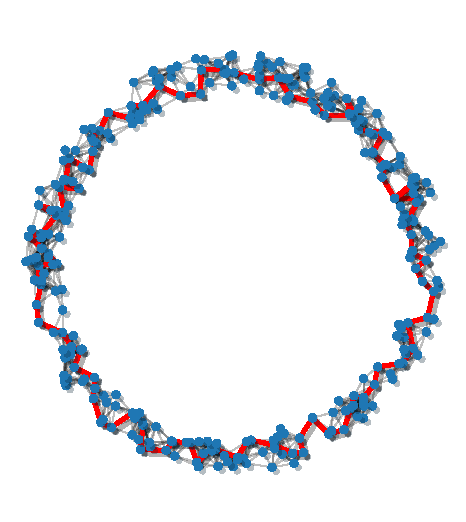
\includegraphics[scale=1.]{figures/homology_cycle.pdf}
    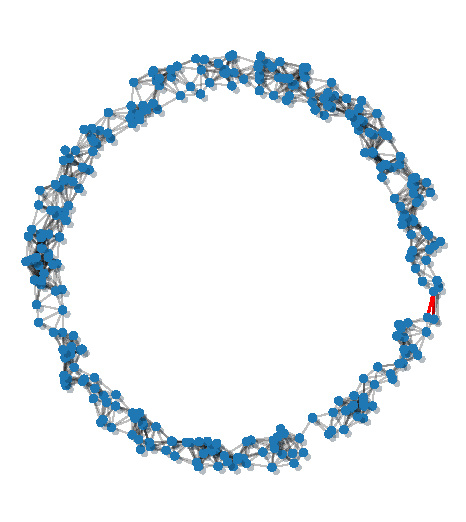
\includegraphics[scale=1.]{figures/cohomology_cocycle.pdf}
    % 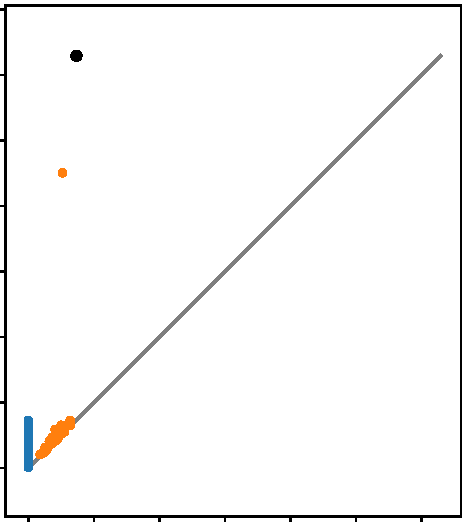
\includegraphics[scale=0.66]{figures/circular_dgm1.pdf}
    \caption{}
    \label{fig:cycles}
\end{figure}

As we will see representative cocycles are particularily useful in distributing the information contained in each Cohomology basis element throughout a simplicial complex.
While this does not have an immediate application to our investigation of coverage in homological sensor network it is a powerful tool which may be used for future research in coordinate free sensor networks.

\subsection{Circular Coordinates}

\begin{figure}[htbp]
\centering
  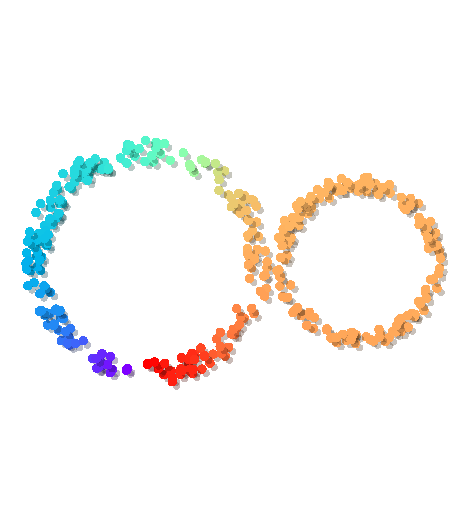
\includegraphics[scale=0.8]{figures/circular_coords1.pdf}
  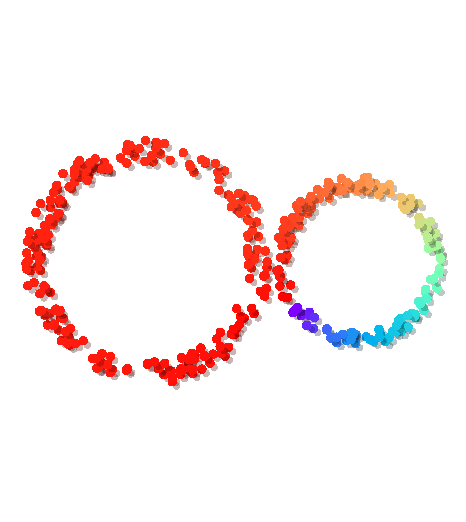
\includegraphics[scale=0.8]{figures/circular_coords2.pdf}\\\vspace{-7ex}
  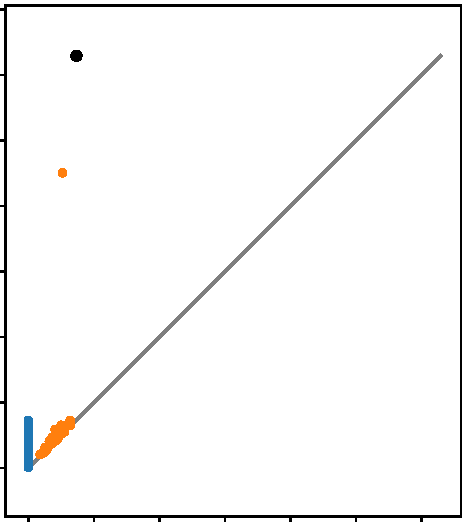
\includegraphics[scale=0.5]{figures/circular_dgm1.pdf}\hspace{1.3in}
  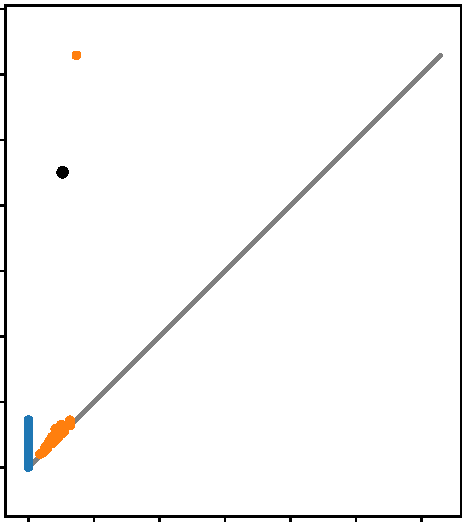
\includegraphics[scale=0.5]{figures/circular_dgm2.pdf}
   \caption{}
   \label{fig:circular}
\end{figure}

\vspace{0.25in}
\textbf{TODO} Cochains as functions on simplicial complexes
\vspace{0.25in}

\subsection{Discrete Exterior Calculus}

% section cohomology (end)
